\documentclass[12pt]{article}
\usepackage{verbatim}
\usepackage[dvips]{epsfig}
\usepackage{color}
\usepackage{url}
\usepackage[colorlinks=true]{hyperref}

\begin{document}

\section*{GENESIS: Documentation}

{\bf Related Documentation:}
% start: userdocs-tag-replace-items related-do-nothing
% end: userdocs-tag-replace-items related-do-nothing

\section*{Rapp: Purkinje Cell Passive Morphology}

\subsection*{Source}

Rapp M, Yarom Y \& Segev I (1994) Physiology, morphology and detailed passive models of guinea-pig cerebellar Purkinje cells. {\it Journal of Physiology} (Lond.). {\bf 474}: 101--118.

\subsection*{Figure}

\begin{figure}[h]
\centering
   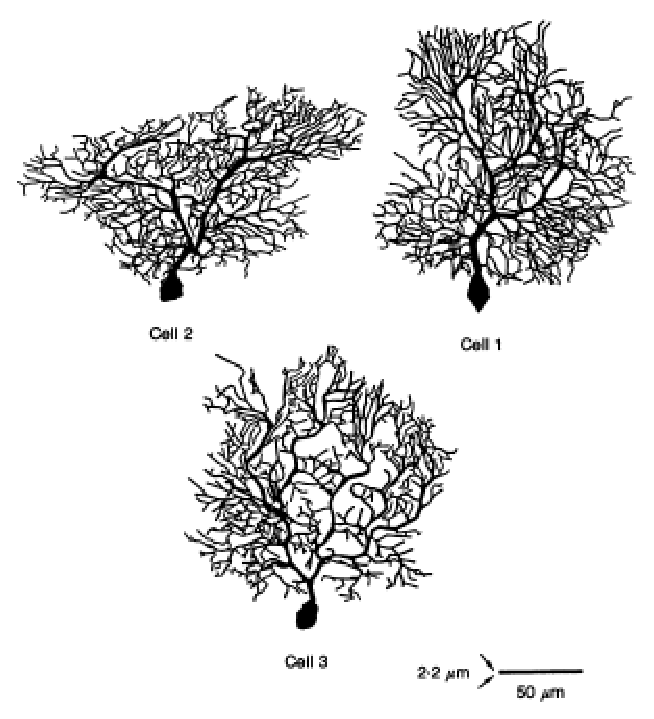
\includegraphics[scale=1]{figures/Fig.3.eps}
   \caption{{\bf Reconstruction of HRP-labelled Purkinje cells from guinea-pig cerebellum.}
Three Purkinje cells were reconstructed in 3D, using a semi-automatic computerized tracing system (Eutectic Inc). Cells were represented by 1400--2100 sample points (each point specified by $x$, $y$ and $z$ coordinates and the diameter of the structure at that point) that were later used to build the corresponding cable and compartmental models. Dendritic spines were not included in this reconstruction but were added to the models assuming that dendritic branches with diameters $<$\,2.2$\mu$m bear 10 spines (um length)$^{-1}$, each spine having an area of 1$\mu$m$^2$. The length of the scale bar represents 50\,$\mu$m of dendritic length whereas the thickness of the scale bar represents 2.2\,$\mu$m dendritic diameter.}
   \label{fig:R.3}
\end{figure}

\bibliographystyle{plain}
\bibliography{../tex/bib/g3-refs}

\end{document}
